\chapter{LeapGesture library dedicated for Leap Motion controller}\label{libraryChapter}

\lstset{ %
language=C++, % choose the language of the code
basicstyle=\footnotesize, % the size of the fonts that are used for the code
numbers=left, % where to put the line-numbers
numberstyle=\footnotesize, % the size of the fonts that are used for the line-numbers
stepnumber=1, % the step between two line-numbers. If it is 1 each line will be numbered
numbersep=5pt, % how far the line-numbers are from the code
backgroundcolor=\color{white}, % choose the background color. You must add \usepackage{color}
showspaces=false, % show spaces adding particular underscores
showstringspaces=false, % underline spaces within strings
showtabs=false, % show tabs within strings adding particular underscores
frame=single, % adds a frame around the code
tabsize=2, % sets default tabsize to 2 spaces
captionpos=b, % sets the caption-position to bottom
breaklines=true, % sets automatic line breaking
breakatwhitespace=false, % sets if automatic breaks should only happen at whitespace
escapeinside={\%*}{*)} % if you want to add a comment within your code
}

A library containing previously described gesture recognition methods has been created.
It is designed as an aid for developers who would like to use gesture input in their applications, but do not want to implement recognition methods manually.
Using it does not require deep knowledge about gesture recognition methods -- a library is like a black box: after initial learning process, it is feed with frames from Leap Motion, and responds if there is a match to previously learnt gesture.
Code was written in C++, so it can be used on many platforms.
When there is a need to use the library in an application written in different programming language, the library can be compiled into dynamic-link library (DLL) or dynamic shared object (DSO) and linked in a project.
Thus, the library can be easily used in many projects.


\section{Architecture} \label{architectureSection}

The library is divided into three main modules:
\begin{itemize}
\item a static gesture recognition module,
\item a dynamic gesture recognition module,
\item a fingers recognition module.
\end{itemize}

Each of those modules has its own separate methods -- for learning new gestures, and for further operational work (recognition). They are implemented using the observer pattern.
The main processing of the library is performed within a separate thread, that creates certain list of events.
The set of observers is defined to be called on the library's events.
The most important events that are fired in the key moments of recognition include: an event when particular gesture began to be recognized, an event when the particular gesture has being recognized, an event when a frame processing is finished.

The library can be divided into learning (offline) and recognition (online) parts.

\subsection{Learning}

Learning process is intended to be run only once and it has to be done before user decides to recognize gestures. Its goal is to create a model, which will be later used in recognition task. As an input, the learning needs a set of recordings. The recordings are files with gestures recorded using the Leap Motion and the Recorder application. Additionally, learning process requires a configuration file containing learning parameters. The output of learning process is a model file used in recognition process.
The learning process informs about the what is the expected recognition rate measured on the training set.

Sample code illustrating the reading recorded data, including the configuration file and performing a process of learning two classes of static gestures:
\begin{lstlisting}
vector<pair<const char*, const char*> > input;
input.push_back(make_pair("gesture1.lmr", "gesture1"));
input.push_back(make_pair("gesture2.lmr", "gesture2"));

TrainingStaticRecConf conf;
conf.configurationPath = "/home/user";
conf.configurationName = "test";

Learning::learnStatic(input, conf);
\end{lstlisting}


\subsection{Testing}

Testing (recognition) process is a process performed to compute if and what gesture is recognized.
The testing process gathers data from the Leap Motion controller and processes them in a separate threads.

\begin{figure}[htb]
\centering
 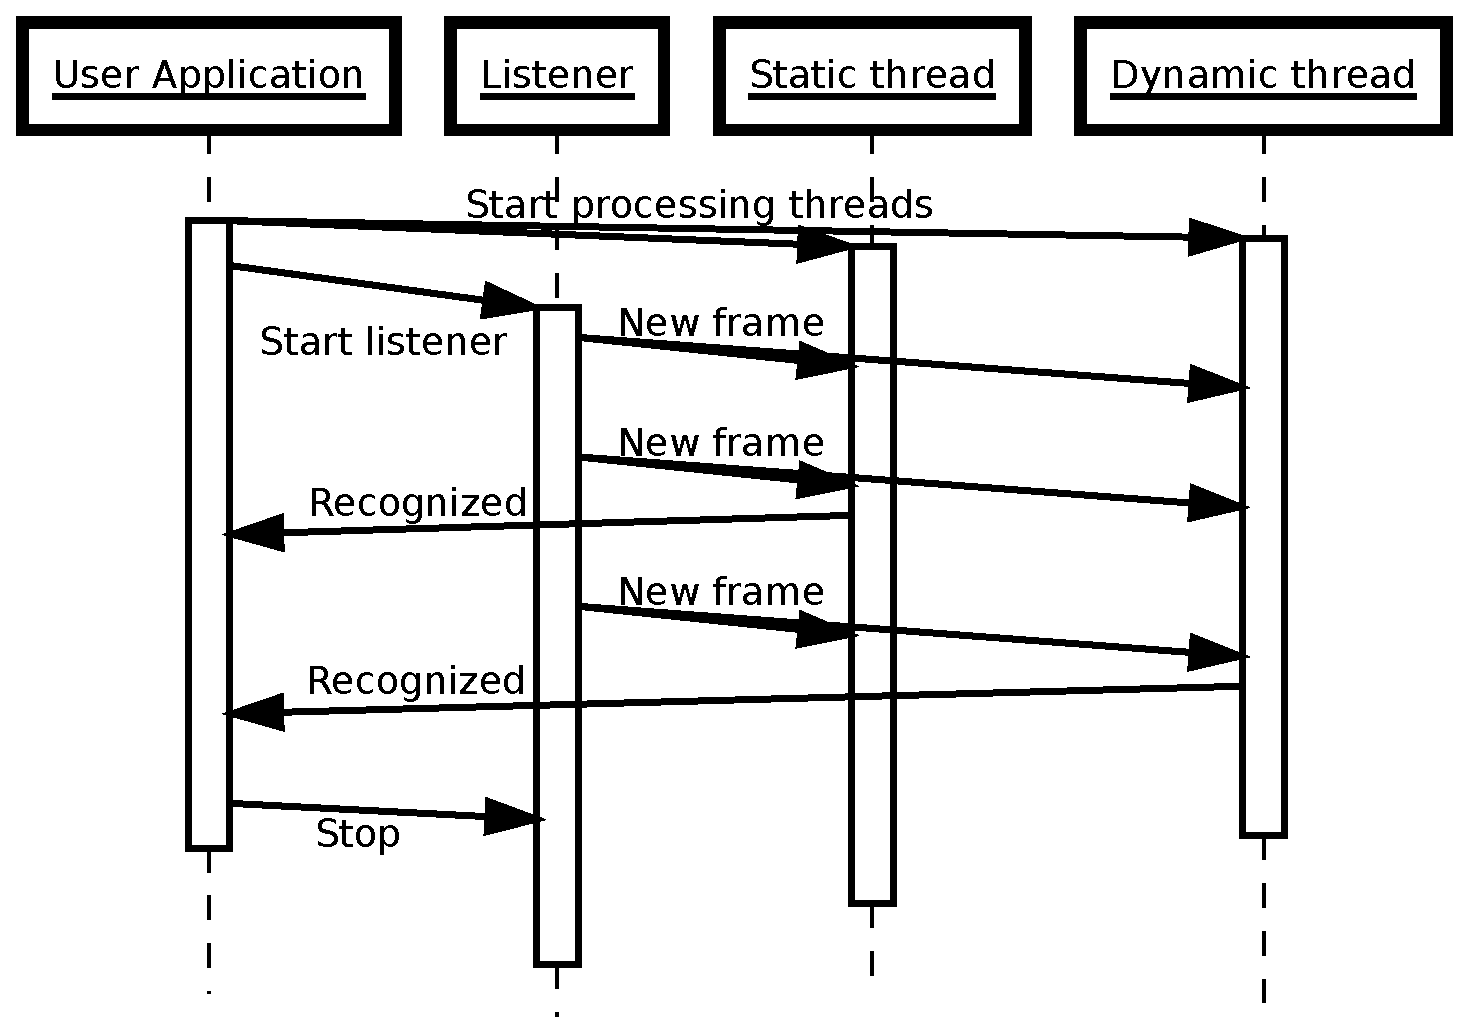
\includegraphics[width=0.8\columnwidth]{figures/timeline.eps}
 \caption[]{Timing diagram of processing static and dynamic gestures}
 \label{processingtimeline}
\end{figure}

The general workflow can be defined in a following way:
\begin{enumerate}
  \item developer creates object of his own class, implementing \texttt{RecognizedGestureListener},
  \item developer creates LeapProcess object, specifies which modules should be run and supplies RecognizedGestureListener object,
  \item developer creates configuration object and sets it as appropriate field in LeapProcess:
  \begin{enumerate}
   \item class TestingStaticRecConf, field staticRecConfiguration -- for static gesture recognition,
   \item class TestingDynamicRecConf, field dynamicRecConfiguration -- for dynamic gesture recognition,
   \item class TestingFingerRecConf, field fingerRecConfiguration -- for fingers recognition,
  \end{enumerate}
  \item developer attaches LeapListener object to the LeapProcess object,
  \item developer starts the process,
  \item if a gesture recognition event had happened, an user supplied method is executed.
\end{enumerate}

Sample code showing testing (recognition) for model prepared in previous step:
\begin{lstlisting}
// specifies method which will be executed after successful recognition
class MyGestures: public RecognizedGestureListener {

void onStaticRecognized(TestingResult *tr) {
if(tr->testClassResults[0].classTrainRate > 0.5) {
cout << "CLASS 0!" << endl;
}
else cout << "CLASS 1!" << endl;
}

void onDynamicRecognized() {}

};

int main(int argc, char **argv) {

// create instance of recognized gesture actions
MyGestures *gst = new MyGestures();

// create new data processor (for static gestures only)
LeapProcess *process = new LeapProcess(gst, true, false);

// specify settings: path where model with given name is located
TestingStaticRecConf settings("/home/user", "test");
process->staticConf = &settings;

// create a listener and attach it to a process
LeapListener listener(3); // 3 = radius of preprocessing windows
listener.attachToProcess(process);

// create a Leap Motion controller object and direct its data output to a listener
Controller c(listener);

// start processing
process->start();

// as processing works in a separate thread, application can now perform other tasks
cin.get();

// stop processing
c.removeListener(listener);

}
\end{lstlisting}

\subsection{Elements of library}



\begin{itemize}
\item LeapProcess -- main class, acting as an interface between Leap Motion device, application and processing threads.
\item LeapListener -- class responsible for gathering data from Leap Motion and feeding them to processing threads (via LeapProcess).
\item FileListener -- as above, but data comes from a file, not controller. Used mainly for testing.
\item TestingResult -- class containing results of testing process:
\begin{itemize}
\item bool recognized -- notifies if a gesture has been recognized
\item string className -- name of class with highest recognition rate
\item string genericClassName -- generic name of class with highest recognition rate
\item vector\textless TestingClassResult \textgreater testClassResults -- vector of TestingClassResult
\end{itemize}
\item TestingClassResult -- contains testing results for a single class
\begin{itemize}
\item double classTrainRate -- recognition rate for given class
\item string className -- name of a classs
\item string genericClassName -- generic name of class
\end{itemize}

\item RecognizedGesture -- abstract class containing methods which will be executed after successful recognition
\item GestureFinger, GestureHand, GestureFrame, Vertex - classes representing respectively: Frame, Hand and Finger, with additional Vertex class, which simpifies operations on 3D points
\item StorageDriver -- class for I/O operations on LMR files
\item LMpre -- class containing data preprocessing methods

\end{itemize}

\subsection{Model}\label{modelSubsection}

While data obtained from Leap Motion Controller are being processed, they are stored using a specially created classes representing the data. The most important class is GestureFrame, which represents a single frame captured from device. All gathered data is stored in a vector containing elements of GestureFrame type. GestureFrame holds the following information:

\begin{itemize}
\item timestamp,
\item list of data of detected hands in the frame, stored in a vector containing elements of GestureHand type.
\end{itemize}

GestureHand stores parameters of hand performing a gesture. In one instance of GestureFrame many instances of GestureHand can be stored. GestureHand holds the following information:
\begin{itemize}
\item hand id,
\item plam position,
\item stabilized palm position,
\item palm normal vector,
\item palm direction vector,
\item list of fingers of particular hand, stored in a vector containing elements GestureFinger type,
\item ordered value, obtained during hand sorting.
\end{itemize}

GestureFinger stores parameters of one finger. In one instance of GestureHand many instances of GestureFinger can be stored. GestureFinger contains:
\begin{itemize}
\item finger id,
\item tip position,
\item stabilized tip position,
\item finger direction vector,
\item finger length,
\item finger width,
\item ordered value, obtained during finger sorting.
\end{itemize}

\subsection{LMR files}\label{lmrFilesSection}
This is a file format specially developed for the LeapGesture library, supported by various modules, i.e., by the visualizer described in Section~\ref{recordvisualSection}. The file structure is as follows:
\begin{itemize}
\item Each line represents one frame.
\item One frame contains: timestamp and hand parameters.
\item Hand parameters include: hand id, palm position, stabilized palm position, palm normal vector, palm direction vector and detected fingers parameters.
\item Finger parameters include: finger id, finger tip position, stabilized tip position, finger direction vector, finger length and finger width.
\end{itemize}

Exemplary lines from a LMR file:
\begin{quote}
{\color{red}4.78984}\#{\color{blue}7 -9.15495;113.759;46.292 0;0;0 -0.157914;-0.981575;0.107585 -0.0196983;-0.105799;-0.994192}f1 {\color{green} -64.0011;122.41;-28.5433 -64.831;125.304;-38.845 -0.574857;0.0254502;-0.817858 50.4269 13.0854}

{\color{red}16.6761}\#{\color{blue}7 -8.94345;113.525;46.2299 0;0;0 -0.158215;-0.981508;0.107745 -0.0193809;-0.106012;-0.994176}f1 {\color{green} -63.8514;122.144;-28.6825 -64.8135;125.248;-38.6638 -0.575861;0.0261358;-0.81713 50.4225 13.0803}

{\color{red}27.4361}\#{\color{blue}7 -8.72478;113.293;46.1443 0;0;0 -0.159539;-0.981183;0.108754 -0.0203256;-0.106877;-0.994065}f1 {\color{green} -63.5346;121.826;-28.7338 -64.7892;125.183;-38.475 -0.576776;0.0265335;-0.816472 50.3783 13.1248}
\end{quote}

This example shows a frame containing a hand with one finger. The color red is used to mark frame timestamp, the blue color
highlights information about hand, and the color green indicates information about the exposed finger.


Technical information regards LMR files:
\begin{itemize}
\item Timestamp and hands are separated by ``\#''.
\item In specified hand occurs hand parameters and fingers.
\item Hand parameters are separated by space, and finger are separated by ``f'' (hands parameters and fingers are separated by ``f'' too).
\item Specified finger has parameters, which are splited by `` ''.
\item Values in the trivalent parameters are separated by a semicolon.
\end{itemize}

\section{Processes}\label{processesSection}

\subsection{The learning process}
The learning process is a process of teaching the LeapGesture library a new gestures by an API user.
Gestures to be learnt are recorded and stored in a LMR format.
The recordings in the LMR format can done using the Gesture Recorder --- a module included in the library, which records data captured by Leap Motion Controller/.
Every LMR file contains only one class of gesture, but each class can be represented by several LMR files.
In the case of static gestures, one recording should represent one gesture recorded at different angles and in the case of dynamic gestures recording should include only one execution of a gesture.

When all desired gestures are prepared, the API user starts the process of learning by calling \texttt{train} method of appropriate module indicating the training set using \texttt{TrainingClassDatasetList} class and the configuration of learning using the object of appropriate configuration class:
\begin{itemize}
\item \texttt{TrainingStaticRecConf} for the static gesture recognition,
\item \texttt{TrainingDynamicRecConf} for the dynamic gesture recognition,
\item \texttt{TrainingFingerRecConf} for the fingers recognition.
\end{itemize}


\begin{figure}[htb]
\centering
 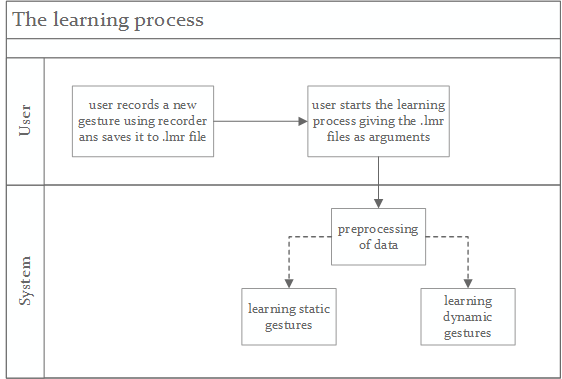
\includegraphics[width=0.75\columnwidth]{figures/learningProcess.png}
 \caption{A diagram presenting the learning process implemented in the LeapGesture library}
 \label{learningprocess}
\end{figure}

Then, the library executes preprocessing on the given training set and starts training, using the selected module by an API user:
\begin{itemize}
\item in case of the static gesture recognition and the fingers recognition modules, the results of training are saved in the MODEL and RANGE files. Those files are needed for proper classification. The former stores learnt model of the Support Vector Machine, the latter contains scaling parameters of learning dataset. In addition, a CLASSMAP file is created, which contains mapping from class names specified by API user to class names supported by the SVM. Some additional files can also be created such as DAT file (raw dataset) or SCALE file (scaled dataset) depending on the established configuration,
\item in case of a dynamic gesture recognition the trained Hidden Markov Models are stored in the HMMMODEL files. The feature scaling is also presented and parameters are stored in the RANGE files. The information to form an observation sequence are stored in file CENTR containing the centroids positions of clusters detected using the k-means algorithm.
\end{itemize}

The library returns information about the outcome of a learning process in the object of \linebreak \texttt{TrainingResult} class.


\subsection{The recognition process}
The recognition process is a process of recognizing the gesture performed by the API user. During this process, the system uses the information obtained from the learning process.

The API user implements \texttt{RecognizedGestureListener} class and creates object of this listener. Then the API user creates an object of \texttt{LeapProcess} class specifying in its constructor which modules should be executed and passes previously initialized object of the listener. The API user also assigns the appropriate configuration object to the corresponding fields of \texttt{LeapProcess} class, which refer to particular modules:
\begin{itemize}
\item for the static gesture recognition the object of \texttt{TestingStaticRecConf} class is assigned to the field \texttt{staticRecConfiguration},
\item for the dynamic gesture recognition the object of \texttt{TestingDynamicRecConf} class is assigned to the field \texttt{dynamicRecConfiguration},
\item for the fingers recognition the object of \texttt{TestingFingerRecConf} class is assigned to the field \texttt{fingerRecConfiguration}.
\end{itemize}
Then the API user adds an object of \texttt{LeapListener} or \texttt{FileListener} to the object of \texttt{LeapProcess} and starts the recognition process.


\begin{figure}[htb]
\centering
 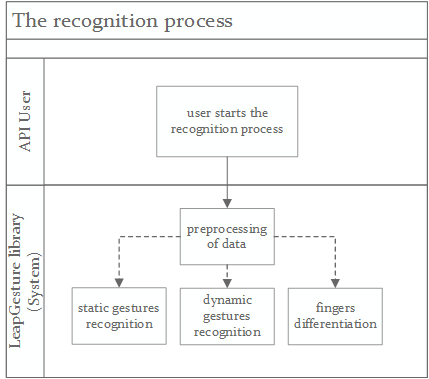
\includegraphics[width=0.6\columnwidth]{figures/recognitionProcess.png}
 \caption{A diagram presenting the recognition process implemented in the LeapGesture library}
 \label{recognitionprocess}
\end{figure}

After the start of recognition process LeapGesture library notifies the object of \linebreak \texttt{RecognizedGestureListener} in case of the occurrence of gestures recognition events.

\section{Gesture recorder and visualizer}\label{recordvisualSection}
The recorder and visualizer module is an additional part of the library that allows users easy management of gestures recordings. The recorder collects data from Leap Motion Controller, converts it into data representation presented in Section~\ref{modelSubsection} and writes it to the LMR file which format is described in Section~\ref{lmrFilesSection}, which is supported by the LeapGesture library. Visualizer enables users to see the recorded gestures stored in LMR format. Data gathered from Leap Motion, used to recognize gestures are very large and the data processed in the library have a specific format. Therefore, it was necessary to create an auxiliary program, that it would facilitate the work with data in the fastest and most user-friendly way.

\subsection{Visualizer}
Visualizer presents the contents of the LMR files. As mentioned earlier, each line of the file is a separately converted frame obtained from Leap Motion Controller. In one moment only one frame is displayed.
Almost all fields of the model are visualized:
\begin{itemize}
\item palm position,
\item palm normal vector,
\item palm direction,
\item tip position,
\item finger direction,
\item finger length.
\end{itemize}

\begin{figure}[htb]
\centering
 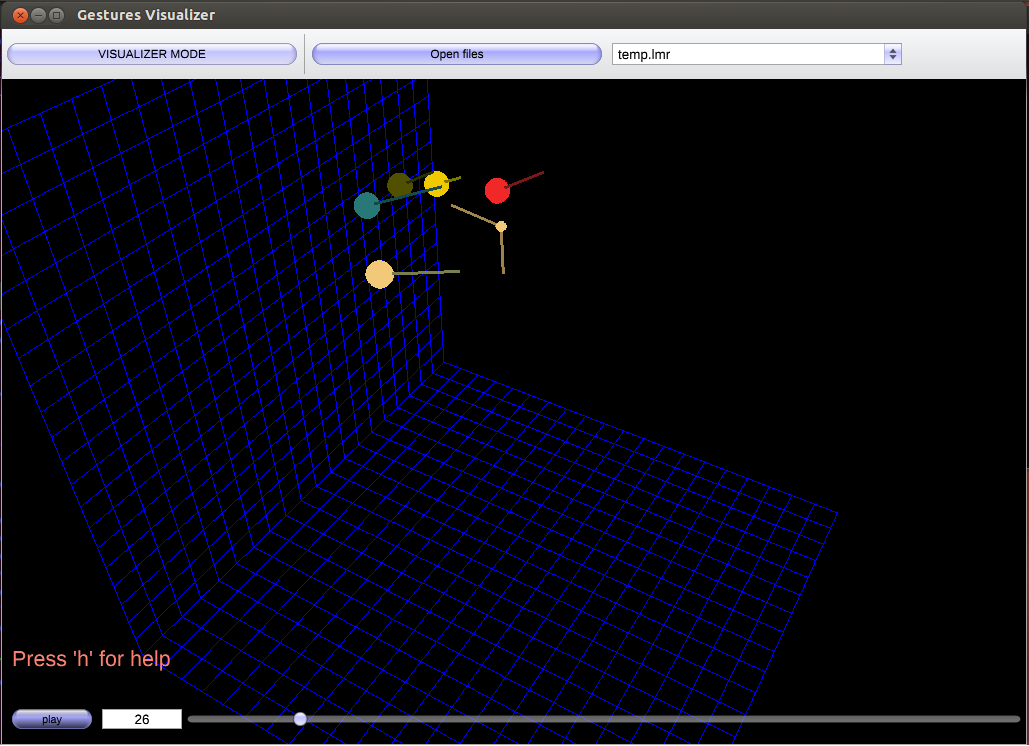
\includegraphics[width=1\columnwidth]{figures/visualizer.png}
 \caption{Screenshot of the visualizer}
 \label{visualizer}
\end{figure}

An example of parameter, which is not visualized, is finger width, in order not to obscure the image.

List of Visualizer features:
\begin{itemize}
\item Program can read the LMR files chosen by the user.
\item The user can load many files at once and select one of the recordings from the drop-down list.
\item To facilitate the user work with visualizer, program has implemented windowing interface.
\item The user has ability to rotate and zoom camera.
\item Slider is available in order to move between frames of the recording.
\item Visualizer has option to play recorded gesture, which the user can turn on and off by pressing the play/stop button.
\item There is also a button to enter the recorder mode.
\end{itemize}

\subsection{Recorder}
Recorder is part of the described module, which is responsible for collecting information from Leap Motion Controller and saving it to LMR file.

\begin{figure}[htb]
\centering
 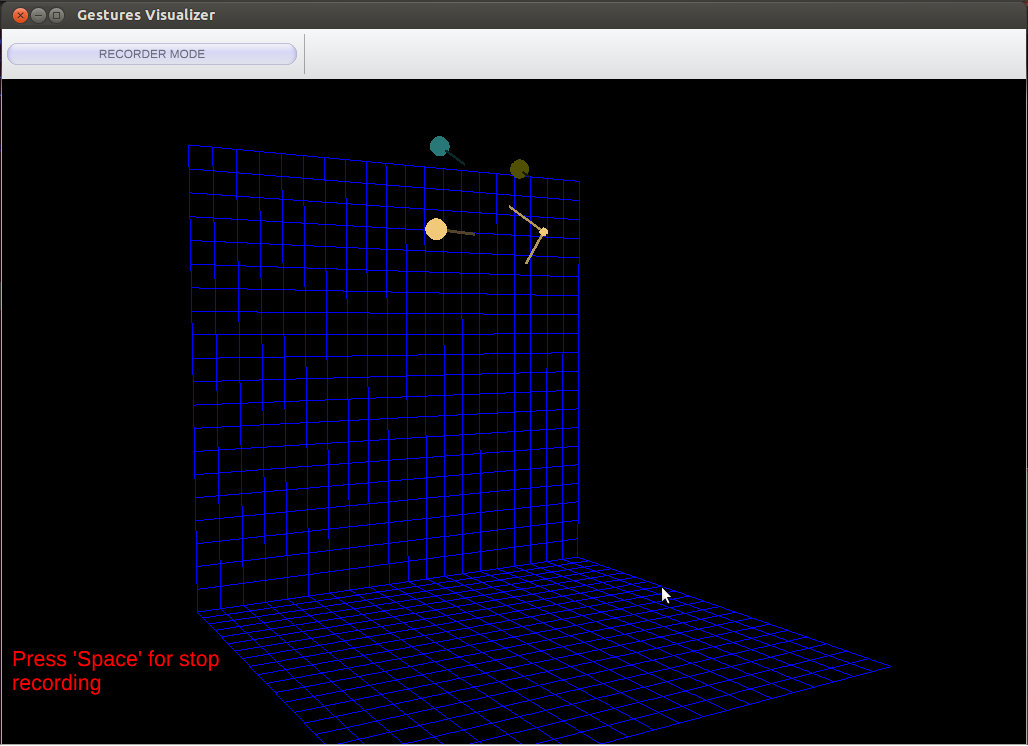
\includegraphics[width=1\columnwidth]{figures/recorder.png}
 \caption{Screenshot of the recorder}
 \label{recorder}
\end{figure}

Each frame read from the Leap Motion is captured, and then converted to the previously described model. Then the model is saved by the appropriate sub-module to LMR file. The conversion process contains also sorting hands and fingers. Hands are sorted by X coordinate of palmPosition. In the case of sorting fingers, the usual sort by the X coordinate is not enough. The order of the fingers must be independent of hand rotation, therefore a different method for fingers sorting had to be proposed. Fingers are sorted by distance between finger tip position and the plane perpendicular to the surface of the hand. The plane has to contain the direction vector of a hand. This plane can be determined using the palm position, the direction vector and a normalized normal vector of the hand.
Below is the formula for the distance ($d$) between finger tip position and designated plane.

\[ d = -(f - pp) \cdot (\hat{hd} \times \hat{hn}) \]
Where:
\begin{itemize}
    \item[] $f$: is the finger tip position
    \item[] $pp$: is the palm position
    \item[] $\hat{hd}$: is a normalized hand direction vector
    \item[] $\hat{hn}$: is a normalized hand normal vector
\end{itemize}

List of Recorder features:
\begin{itemize}
\item Turning on and off recording is done by using space key.
\item After recording window automatically appears, in which can be choosen where to save the file.
\item The recorder cooperates with the visualizer. During recording performed gesture is visualized.
\item There is a button to enter the visualizer mode.
\end{itemize}

\section{External libraries used} \label{librariesSection}

\begin{itemize}
\item LeapSDK -- allows to access Leap Motion device and its API
\item pthread -- library used to create lightweight processes (threads), to allow simulteanous (multithreaded) processing and provide task synchronization
\item LIBSVM -- ''A Library for Support Vector Machines'', provides SVM classifying algorithm,
\item Dlib -- provides k--means clustering, Chinese Whispers and Newman's Clustering algorithms,
\item HMMlib -- a C++ library containing optimized version of the Hidden Markov Models,
\item Boost -- C++ extensions library, provides smart pointer mechanism for HMMlib.
\end{itemize}
